\documentclass{standalone}
\usepackage{tikz}
\usetikzlibrary{patterns, positioning}
\usepackage[sfdefault]{ClearSans} %% option 'sfdefault' activates Clear Sans as the default text font
\usepackage[T1]{fontenc}

\begin{document}
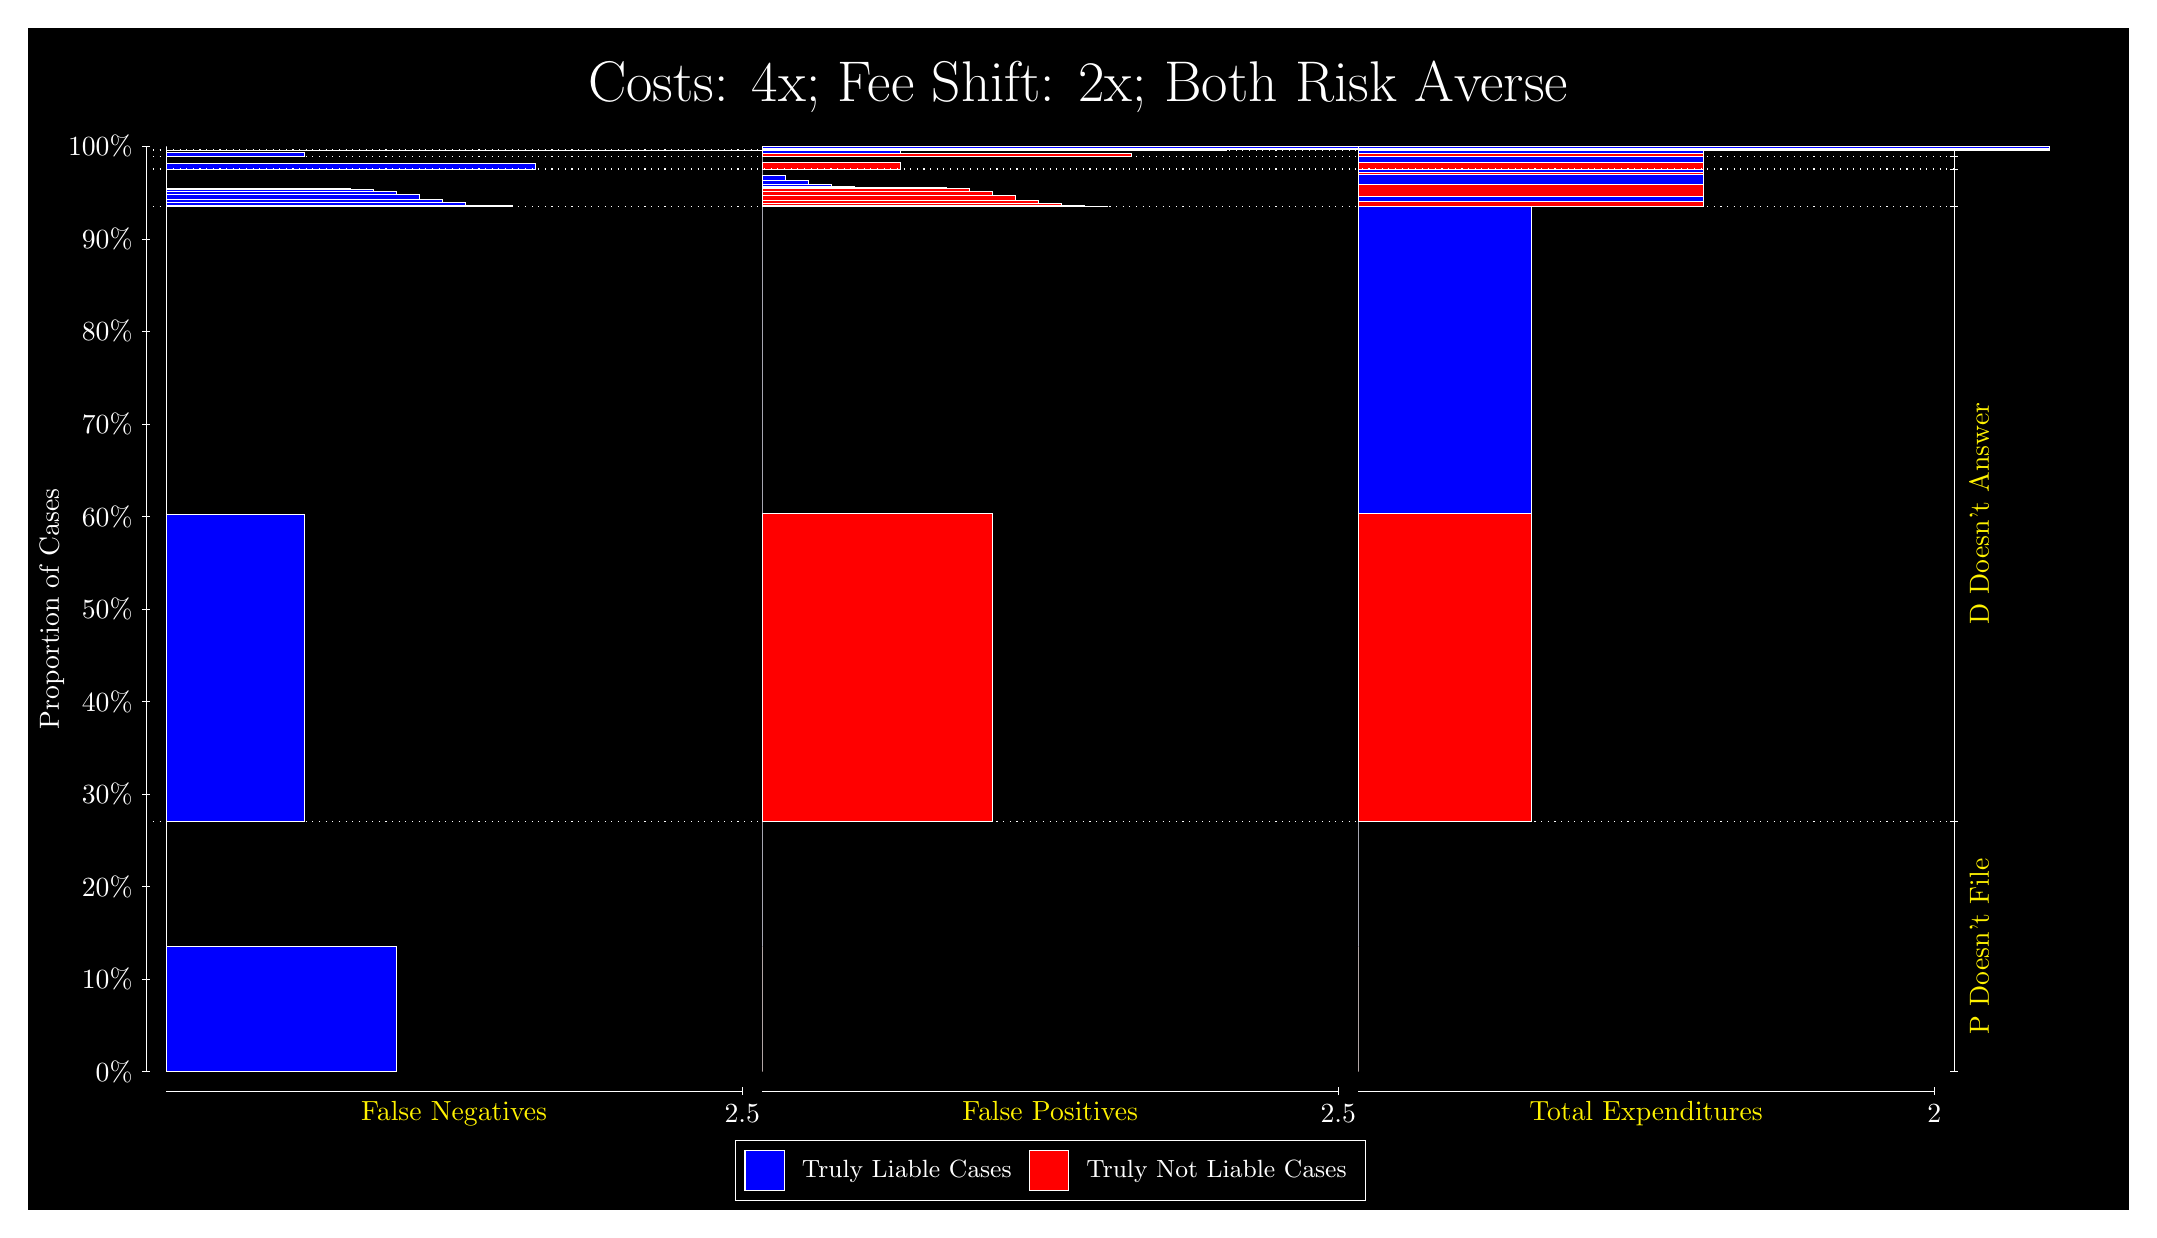
\begin{tikzpicture}
\draw[fill=black] (0,0) rectangle (26.667,15);
\draw[text=white] (0,13.5) rectangle (26.667,15) node[midway] {\huge Costs: 4x; Fee Shift: 2x; Both Risk Averse};
\draw[white, very thin] (1.5,1.75) -- (1.5,13.5);
\node[rotate=90, text=white, anchor=center] at (0.3, 7.625) {Proportion of Cases};
\draw[white, very thin] (1.45,1.75) -- (1.55,1.75);
\node[text=white, anchor=east] at (1.45, 1.75) {0\%};
\draw[white, very thin] (1.45,2.925) -- (1.55,2.925);
\node[text=white, anchor=east] at (1.45, 2.925) {10\%};
\draw[white, very thin] (1.45,4.1) -- (1.55,4.1);
\node[text=white, anchor=east] at (1.45, 4.1) {20\%};
\draw[white, very thin] (1.45,5.275) -- (1.55,5.275);
\node[text=white, anchor=east] at (1.45, 5.275) {30\%};
\draw[white, very thin] (1.45,6.45) -- (1.55,6.45);
\node[text=white, anchor=east] at (1.45, 6.45) {40\%};
\draw[white, very thin] (1.45,7.625) -- (1.55,7.625);
\node[text=white, anchor=east] at (1.45, 7.625) {50\%};
\draw[white, very thin] (1.45,8.8) -- (1.55,8.8);
\node[text=white, anchor=east] at (1.45, 8.8) {60\%};
\draw[white, very thin] (1.45,9.975) -- (1.55,9.975);
\node[text=white, anchor=east] at (1.45, 9.975) {70\%};
\draw[white, very thin] (1.45,11.15) -- (1.55,11.15);
\node[text=white, anchor=east] at (1.45, 11.15) {80\%};
\draw[white, very thin] (1.45,12.325) -- (1.55,12.325);
\node[text=white, anchor=east] at (1.45, 12.325) {90\%};
\draw[white, very thin] (1.45,13.5) -- (1.55,13.5);
\node[text=white, anchor=east] at (1.45, 13.5) {100\%};

\draw[white, very thin] (24.457,1.75) -- (24.457,13.5);
\draw[white, very thin] (24.407,1.75) -- (24.507,1.75);
\node[anchor=west] at (24.407, 1.75) {};
\draw[white, very thin] (24.407,4.9296) -- (24.507,4.9296);
\node[anchor=west] at (24.407, 4.9296) {};
\draw[white, very thin] (24.407,12.739) -- (24.507,12.739);
\node[anchor=west] at (24.407, 12.739) {};
\draw[white, very thin] (24.407,13.212) -- (24.507,13.212);
\node[anchor=west] at (24.407, 13.212) {};
\draw[white, very thin] (24.407,13.374) -- (24.507,13.374);
\node[anchor=west] at (24.407, 13.374) {};
\draw[white, very thin] (24.407,13.453) -- (24.507,13.453);
\node[anchor=west] at (24.407, 13.453) {};
\draw[white, very thin] (24.407,13.465) -- (24.507,13.465);
\node[anchor=west] at (24.407, 13.465) {};
\draw[white, very thin] (24.407,13.5) -- (24.507,13.5);
\node[anchor=west] at (24.407, 13.5) {};

\draw[white, very thin, fill=blue] (1.75,1.75) rectangle (4.6775,3.3398);
\draw[white, very thin, fill=red] (1.75,3.3398) rectangle (1.75,4.9296);
\draw[white, very thin, fill=blue] (1.75,4.9296) rectangle (3.5065,8.833);
\draw[white, very thin, fill=red] (1.75,8.833) rectangle (1.75,12.739);
\draw[white, very thin, fill=blue] (1.75,12.739) rectangle (6.1413,12.747);
\draw[white, very thin, fill=blue] (1.75,12.747) rectangle (5.8486,12.753);
\draw[white, very thin, fill=blue] (1.75,12.753) rectangle (5.5558,12.784);
\draw[white, very thin, fill=blue] (1.75,12.784) rectangle (5.2631,12.822);
\draw[white, very thin, fill=blue] (1.75,12.822) rectangle (4.9703,12.887);
\draw[white, very thin, fill=blue] (1.75,12.887) rectangle (4.6775,12.93);
\draw[white, very thin, fill=blue] (1.75,12.93) rectangle (4.3848,12.96);
\draw[white, very thin, fill=blue] (1.75,12.96) rectangle (4.092,12.966);
\draw[white, very thin, fill=blue] (1.75,12.966) rectangle (3.7993,12.971);
\draw[white, very thin, fill=red] (1.75,12.971) rectangle (1.75,13.212);
\draw[white, very thin, fill=blue] (1.75,13.212) rectangle (6.4341,13.284);
\draw[white, very thin, fill=red] (1.75,13.284) rectangle (1.75,13.374);
\draw[white, very thin, fill=blue] (1.75,13.374) rectangle (3.5065,13.419);
\draw[white, very thin, fill=red] (1.75,13.419) rectangle (1.75,13.453);
\draw[white, very thin, fill=blue] (1.75,13.453) rectangle (15.217,13.455);
\draw[white, very thin, fill=red] (1.75,13.455) rectangle (1.75,13.465);
\draw[white, very thin, fill=red] (1.75,13.465) rectangle (1.75,13.469);
\draw[white, very thin, fill=blue] (1.75,13.469) rectangle (1.75,13.5);
\draw[white, very thin, fill=red] (9.3189,1.75) rectangle (9.3189,3.3398);
\draw[white, very thin, fill=blue] (9.3189,3.3398) rectangle (9.3189,4.9296);
\draw[white, very thin, fill=red] (9.3189,4.9296) rectangle (12.246,8.8361);
\draw[white, very thin, fill=blue] (9.3189,8.8361) rectangle (9.3189,12.739);
\draw[white, very thin, fill=red] (9.3189,12.739) rectangle (13.71,12.744);
\draw[white, very thin, fill=red] (9.3189,12.744) rectangle (13.417,12.749);
\draw[white, very thin, fill=red] (9.3189,12.749) rectangle (13.125,12.774);
\draw[white, very thin, fill=red] (9.3189,12.774) rectangle (12.832,12.82);
\draw[white, very thin, fill=red] (9.3189,12.82) rectangle (12.539,12.883);
\draw[white, very thin, fill=red] (9.3189,12.883) rectangle (12.246,12.931);
\draw[white, very thin, fill=red] (9.3189,12.931) rectangle (11.954,12.968);
\draw[white, very thin, fill=red] (9.3189,12.968) rectangle (11.661,12.974);
\draw[white, very thin, fill=red] (9.3189,12.974) rectangle (11.368,12.981);
\draw[white, very thin, fill=blue] (9.3189,12.981) rectangle (10.783,12.985);
\draw[white, very thin, fill=blue] (9.3189,12.985) rectangle (10.49,12.992);
\draw[white, very thin, fill=blue] (9.3189,12.992) rectangle (10.197,13.022);
\draw[white, very thin, fill=blue] (9.3189,13.022) rectangle (9.9044,13.065);
\draw[white, very thin, fill=blue] (9.3189,13.065) rectangle (9.6116,13.13);
\draw[white, very thin, fill=blue] (9.3189,13.13) rectangle (9.3189,13.212);
\draw[white, very thin, fill=red] (9.3189,13.212) rectangle (11.075,13.302);
\draw[white, very thin, fill=blue] (9.3189,13.302) rectangle (9.3189,13.374);
\draw[white, very thin, fill=red] (9.3189,13.374) rectangle (14.003,13.408);
\draw[white, very thin, fill=blue] (9.3189,13.408) rectangle (11.075,13.453);
\draw[white, very thin, fill=red] (9.3189,13.453) rectangle (9.3189,13.463);
\draw[white, very thin, fill=blue] (9.3189,13.463) rectangle (9.3189,13.465);
\draw[white, very thin, fill=red] (9.3189,13.465) rectangle (22.786,13.469);
\draw[white, very thin, fill=blue] (9.3189,13.469) rectangle (19.858,13.5);
\draw[white, very thin, fill=red] (16.888,1.75) rectangle (16.888,3.3398);
\draw[white, very thin, fill=blue] (16.888,3.3398) rectangle (16.888,4.9296);
\draw[white, very thin, fill=red] (16.888,4.9296) rectangle (19.083,8.8361);
\draw[white, very thin, fill=blue] (16.888,8.8361) rectangle (19.083,12.739);
\draw[white, very thin, fill=red] (16.888,12.739) rectangle (21.279,12.803);
\draw[white, very thin, fill=blue] (16.888,12.803) rectangle (21.279,12.868);
\draw[white, very thin, fill=red] (16.888,12.868) rectangle (21.279,13.016);
\draw[white, very thin, fill=blue] (16.888,13.016) rectangle (21.279,13.146);
\draw[white, very thin, fill=red] (16.888,13.146) rectangle (21.279,13.176);
\draw[white, very thin, fill=blue] (16.888,13.176) rectangle (21.279,13.212);
\draw[white, very thin, fill=red] (16.888,13.212) rectangle (21.279,13.302);
\draw[white, very thin, fill=blue] (16.888,13.302) rectangle (21.279,13.374);
\draw[white, very thin, fill=red] (16.888,13.374) rectangle (21.279,13.408);
\draw[white, very thin, fill=blue] (16.888,13.408) rectangle (21.279,13.453);
\draw[white, very thin, fill=red] (16.888,13.453) rectangle (25.67,13.463);
\draw[white, very thin, fill=blue] (16.888,13.463) rectangle (25.67,13.465);
\draw[white, very thin, fill=red] (16.888,13.465) rectangle (25.67,13.469);
\draw[white, very thin, fill=blue] (16.888,13.469) rectangle (25.67,13.5);
\draw[white, dotted] (1.5,4.9296) -- (24.457,4.9296);
\draw[white, dotted] (1.5,12.739) -- (24.457,12.739);
\draw[white, dotted] (1.5,13.212) -- (24.457,13.212);
\draw[white, dotted] (1.5,13.374) -- (24.457,13.374);
\draw[white, dotted] (1.5,13.453) -- (24.457,13.453);
\draw[white, dotted] (1.5,13.465) -- (24.457,13.465);
\draw[white, very thin] (1.75,1.5) -- (9.0689,1.5);
\node[text=yellow, anchor=north] at (5.4094, 1.5) {False Negatives};
\draw[white, very thin] (9.0689,1.45) -- (9.0689,1.55);
\node[text=white, anchor=north] at (9.0689, 1.45) {2.5};

\draw[white, very thin] (9.3189,1.5) -- (16.638,1.5);
\node[text=yellow, anchor=north] at (12.978, 1.5) {False Positives};
\draw[white, very thin] (16.638,1.45) -- (16.638,1.55);
\node[text=white, anchor=north] at (16.638, 1.45) {2.5};

\draw[white, very thin] (16.888,1.5) -- (24.207,1.5);
\node[text=yellow, anchor=north] at (20.547, 1.5) {Total Expenditures};
\draw[white, very thin] (24.207,1.45) -- (24.207,1.55);
\node[text=white, anchor=north] at (24.207, 1.45) {2};

\node[text=yellow, centered, rotate=90] at (24.777, 3.3398) {P Doesn't File};
\node[text=yellow, centered, rotate=90] at (24.777, 8.8345) {D Doesn't Answer};






\draw (12.978300999999998,1.5) node[draw=none] (baseCoordinate) {};
\begin{scope}[align=center]
        \matrix[scale=0.5, draw=white, below=0.5cm of baseCoordinate, nodes={draw}, column sep=0.1cm]{
            \node[rectangle, draw, minimum width=0.5cm, minimum height=0.5cm, fill=blue] {}; &
            \node[draw=none, font=\small, text=white] (B) {Truly Liable Cases}; &
            \node[rectangle, draw, minimum width=0.5cm, minimum height=0.5cm, fill=red] {}; &
            \node[draw=none, font=\small, text=white] (B) {Truly Not Liable Cases}; \\
            };
\end{scope}

\end{tikzpicture}
\end{document}